\documentclass[tikz,border=10pt]{standalone}
\usepackage[utf8]{vietnam}
\usepackage{amsmath,amssymb}
\usepackage{tkz-euclide,tkz-tab,pgfplots}
\pgfplotsset{compat=newest}
\usetikzlibrary{math,through,calc,fadings,intersections,shadings,angles,quotes,shapes,shapes.geometric,arrows,patterns,snakes,decorations.text,matrix,chains}
%\usetkzobj{all}
\begin{document}
	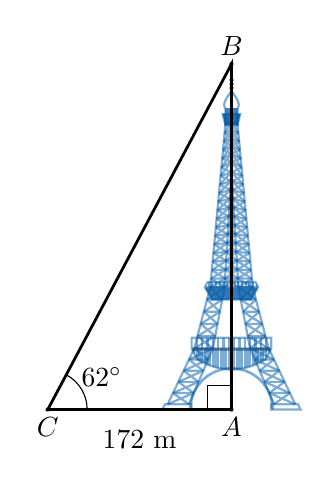
\begin{tikzpicture}[scale=0.5] % Tăng scale tổng thể lên một chút để dễ nhìn
	% Tháp Eiffel
	% Bỏ đi phần shift={...current page...} để tránh bị lệch hình ngoài trang
	\begin{scope}[thick,scale=.27,blue!30!teal,opacity=0.5]
	\fill[blue!30!teal] (180:3.75) arc (180:0:3.75)--(0:4) arc (0:180:4)--cycle;
	\path (0,0) coordinate (TA);
	\foreach \xsc/\t in {1/A,-1/B}{
		\begin{scope}[xscale=\xsc]% Đế và thân tháp
		\draw (3.75,0) -- (6.5,0)--(6.25,.5)--(3.75,.5)--cycle;% Đế
		\draw 
		(6,.5)--(3.5,5.75)\foreach \x[count=\i from 0] in {0,.2,...,1}{coordinate[pos=\x](\t1\i)}
		--(2,11.5)\foreach \x[count=\i from 6] in {.2,.4,...,1}{coordinate[pos=\x](\t1\i)}
		--(.5,27.6) \foreach \x[count=\i from 11] in {.05,.1,...,1}{coordinate[pos=\x](\t1\i)}
		(4,.5)--(1.75,5.75)\foreach \x[count=\i from 0] in {0,.2,...,1}{coordinate[pos=\x](\t2\i)}
		--(.65,11.5)\foreach \x[count=\i from 6] in {.2,.4,...,1}{coordinate[pos=\x](\t2\i)}
		--(0,22.6)\foreach \x[count=\i from 11] in {.075,.15,...,1}{coordinate[pos=\x](\t2\i)}
		--(0,27.6)\foreach \x[count=\i from 24] in {.15,.3,...,1}{coordinate[pos=\x](\t2\i)}
		;
		\end{scope}
	}
	%%%%%% Các đường nối
	\foreach \i in {0,...,28}{
		\pgfmathsetmacro\j{int(\i+1)}
		\draw 
		(A1\i)--(A2\j) (A2\i)--(A1\j) (A1\j)--(A2\j)
		(B1\i)--(B2\j) (B2\i)--(B1\j) (B1\j)--(B2\j)
		;
	}
	\foreach \i in {10,...,28}{
		\pgfmathsetmacro\j{int(\i+1)}
		\draw (A2\i)--(B2\j) (A2\j)--(B2\i) (A2\j)--(B2\j);
	}
	%%%%%%%%%%%%
	\begin{scope}% Tầng 1
		\draw 
		(-3.75,5.75) rectangle +(7.5,1)
		(-3.75,5.75)--($(B14)!.1!(A14)$) to[out=-30,in=-150] ($(A14)!.1!(B14)$)--(3.75,5.75)
		;
		\fill[black!75] (-3.75,5.75) rectangle +(7.5,-.25);
		\foreach \x in {-3.25,-2.75,...,3.25}\draw[thick] (\x,5.75)--++(0,1);
		\clip (-3.75,5.75)--($(B14)!.1!(A14)$) to[out=-30,in=-150] ($(A14)!.1!(B14)$)--(3.75,5.75);
		\foreach \x in {-3.5,-3.25,...,3.5}\draw (\x,5.75)--++(0,-2);
	\end{scope}
	\begin{scope}% Tầng 2
		\draw (2.5,11.5)--(-2.5,11.5)
		(2.5,11.5)--(2.25,12)--(-2.25,12)--(-2.5,11.5)--($(B19)!.1!(A19)$)--($(A19)!.1!(B19)$)--cycle;
		\begin{scope}
			\clip (2.5,11.5)--(-2.5,11.5)--($(B19)!.1!(A19)$)--($(A19)!.1!(B19)$)--cycle;
			\foreach \x in {-3.25,-3,...,3.25}\draw (\x,11.5)--++(-45:3) (\x,11.5)--++(-135:3);
		\end{scope}
		\begin{scope}
			\clip (-2.5,11.5)--(-2.25,12)--(2.25,12)--(2.5,11.5)--cycle;
			\foreach \x in {-2.5,-2.15,...,2.5}\draw (\x,11.5)--++(0,1);
		\end{scope}
	\end{scope}
	\begin{scope}% Đỉnh
		\draw (A129)--(B129)--($(B129)+(-.25,1)$)--($(A129)+(.25,1)$)--cycle;
		\clip (A129)--(B129)--($(B129)+(-.25,1)$)--($(A129)+(.25,1)$)--cycle;
		\foreach \x in {-3,-2.8,...,3}\draw (\x,26)--++(45:3) (\x,26)--++(135:3);
	\end{scope}
	\begin{scope}% Chóp
		\draw (A129)--+(0,1.5) to[out=60,in=-60] (0,30) to[out=-120,in=120]($(B129)+(0,1.5)$)--(B129)
		(0,27.6)--(0,32.5) coordinate (TB);
		\fill[black] 
		(0,30.25) ellipse ({.25} and {.1})
		(0,30.6) ellipse ({.25} and {.1})
		(0,31) ellipse ({.25} and {.1})
		;
		\clip ($(A129)+(0,1)$)--($(B129)+(0,1)$)--++(0,.5)--($(A129)+(0,1.5)$);
		\foreach \y in {27,27.1,...,32}\draw (-2,\y)--(2,\y);
	\end{scope}
	\end{scope}
	
	% ==============================================
	% PHẦN CẬP NHẬT: Gán tam giác ABC vào đúng tháp
	% ==============================================
	\coordinate (A) at (TA); % A nằm đúng chính giữa chân tháp
	\coordinate (B) at (TB); % B nằm đúng đỉnh chóp của tháp
	
	% Đặt C sao cho hợp với đường cao tháp thành tam giác vuông chuẩn (tan(62) tính tay là phù hợp)
	\coordinate (C) at (-4.666, 0); 
	
	\draw[line width=1pt] (A)--(B)--(C)--cycle;
	\draw pic[draw, angle radius=5mm, angle eccentricity=1.6, "$62^\circ$"]{angle = A--C--B};
	\draw pic[draw, angle radius=3mm]{right angle = B--A--C};
	
	\path (A)--(C) node[midway, below=0.15] {$172$ m};
	
	% Đặt text A, B, C cho hợp lý
	\foreach \x/\y in {A/-90, B/90, C/-90}{
		\fill (\x) circle (1.5pt);
		\node at ($(\x)+(\y:0.45cm)$) {$\x$};
	}
\end{tikzpicture}
\end{document}